% Compile: pdflatex supplementary x2
\documentclass[11pt]{article}
\usepackage{graphicx}
\usepackage{amsmath}
\usepackage{amssymb}
\usepackage{xcolor}
\usepackage{booktabs}
\usepackage[margin=1in]{geometry}
\usepackage{placeins}
\usepackage{algorithm}
\usepackage{algpseudocode}
\usepackage[colorlinks=true, linkcolor=blue, citecolor=blue, urlcolor=blue]{hyperref}

\renewcommand{\thesection}{S\arabic{section}}
\renewcommand{\thetable}{S\arabic{table}}
\renewcommand{\thefigure}{S\arabic{figure}}
\renewcommand{\theequation}{S\arabic{equation}}
\makeatletter\AtBeginDocument{\renewcommand{\thealgorithm}{S\arabic{algorithm}}}\makeatother

\setlength{\parskip}{0.5em}
\setlength{\parindent}{1.5em}

\title{Supplementary Information for \\ ``Projections of Earth's Technosphere: \\ Civilization Collapse--Recovery Dynamics and Detectability''}
\author{Celia Blanco, Jacob Haqq-Misra, George Profitiliotis}
\date{}

\begin{document}
\maketitle

\section{Simulation pseudocode}\label{app:pseudocode}

Algorithm~\ref{alg:sim} summarizes the complete simulation sequence for one Monte Carlo replicate, covering parameter sampling, growth, resource consumption, hazard events, collapse, dormant recovery, partial restoration, and the calculation of the outcome metrics.

\begin{algorithm}[htbp]
\caption{Collapse-recovery simulation for one Monte Carlo replicate}
\label{alg:sim}
\begin{algorithmic}[1]
\State Sample $R_0, \delta, c_f, r_d, r_f$ from scenario-specific distributions (Table~5 of the main text), truncated to admissible ranges
\State Initialize $T \gets 1$, $R \gets R_0$, state $\gets$ \textsc{active}
\For{$t = 1, \dots, T_{\mathrm{span}}$}
    \If{state $=$ \textsc{active}}
        \State $T \gets T + r$; \quad $R \gets R - \delta$ \Comment{growth and consumption}
        \State draw $U \sim U(0,1)$; if $U < h$ then $R \gets 0$ \Comment{external hazard}
        \If{$R \leq 0$} \Comment{collapse (depletion or hazard)}
            \State $R \gets 0$; \quad $T \gets c_f\, T$; \quad state $\gets$ \textsc{dormant}; \quad timer $\gets 0$
        \EndIf
    \Else \Comment{dormant recovery phase}
        \State timer $\gets$ timer $+ 1$
        \If{timer $\geq r_d$}
            \State $R \gets r_f R_0$; \quad state $\gets$ \textsc{active} \Comment{partial restoration}
        \EndIf
    \EndIf
    \State record $T(t)$, $R(t)$, collapse events and their trigger
\EndFor
\State compute metrics $T_c$, $N_c$, $D_c$ (Section~3.3 of the main text)
\end{algorithmic}
\end{algorithm}

\FloatBarrier

\section{Parameter rationale by scenario}\label{app:rationale}

Table~\ref{tab:rationale} states, for each scenario, the narrative basis on which each parameter value in Table~4 of the main text was assigned, complementing the governance and resource-pressure logic of Tables~2 and 3 of the main text. The growth rate $r$ is in all cases taken directly from Haqq-Misra et al.\ (2025), Table~9, and is not re-derived here. We reiterate that these are exploratory, internally consistent assignments rather than empirical estimates; the plausible ranges explored around them are given in Table~5 of the main text (local uncertainty) and Table~6 of the main text together with Supplementary Figure~\ref{fig:gsa} (global ranges).

\begin{table*}[htbp]
\centering
\caption{Narrative rationale for scenario parameter assignments.}
\label{tab:rationale}
\small
\setlength{\tabcolsep}{5pt}
\renewcommand{\arraystretch}{1.3}
{\raggedright
\begin{tabular}{l p{4.6cm} p{5.2cm} p{3.6cm}}
\toprule
Scenario & Resource regime ($R_0$, $\delta$) & Collapse and recovery ($c_f$, $r_d$, $r_f$) & Aggregate hazard exposure ($h$) \\
\midrule
S1 & Scarcity under authoritarian extraction: low stock (400), elevated depletion (1.2). & Concentrated infrastructure retains capacity ($c_f{=}0.6$, upper rule-by-one range); top-down coordination recovers quickly ($r_d{=}40$); weak societal buy-in limits replenishment ($r_f{=}0.15$). & Elevated exposure through unstable geopolitics: $h{=}0.003$. \\
S2 & Competitive, deregulated extraction: moderate stock (700), high depletion (1.5). & Fragmented coordination deepens collapse ($c_f{=}0.3$) and slows rebuilding ($r_d{=}70$); weak institutional memory ($r_f{=}0.10$). & Moderate exposure: conflict-prone but decentralized ($h{=}0.001$). \\
S3 & Post-scarcity idealization: abundant stock (2400), no net depletion ($\delta{=}0$). & No-collapse limit: $c_f{=}1$, $r_d{=}0$, $r_f{=}1$. & No exogenous exposure channel: stable society ($h{=}0$). \\
S4 & Ecologically constrained cyclical society: modest stock (600), highest depletion relative to regeneration (2.5). & Low-complexity infrastructure lost deeply in collapse ($c_f{=}0.2$); slow agrarian rebuilding ($r_d{=}100$, $r_f{=}0.10$). & Minimal exposure surface: low-impact lifestyle ($h{=}0$). \\
S5 & Post-biological abundance: large stock (2500), minimal depletion (0.1). & Digital redundancy preserves capacity ($c_f{=}0.9$); rapid reconstitution ($r_d{=}20$, $r_f{=}0.80$). & Residual exposure through systemic complexity ($h{=}0.0005$). \\
S6 & Large stock (1600) under sustained high-tech extraction (1.0): scarcity through pressure, not endowment. & Cascading interdependent failures ($c_f{=}0.4$, $r_d{=}50$, $r_f{=}0.25$). & Largest engineered exposure surface: tightly coupled high-risk systems ($h{=}0.005$). \\
S7 & Post-collapse rebuilding: reduced effective stock (400), moderate-high depletion (1.5), overriding the nominal non-scarcity tag (see Section~3.2 of the main text). & Distributed institutions rebuilding from prior damage ($c_f{=}0.3$, $r_d{=}60$, $r_f{=}0.20$). & Residual exposure during rebuilding: $h{=}0.001$. \\
S8 & Oscillatory regime: moderate stock (800) and depletion (1.3) tuned so cycles emerge endogenously. & Partial technological survival ($c_f{=}0.6$) with substantial resource regeneration ($r_f{=}0.35$, $r_d{=}70$), sustaining repeated cycles. & No exogenous exposure channel: collapse endogenous by construction ($h{=}0$). \\
S9 & Aggressive expansion drives extraction despite nominal post-scarcity: stock 900, depletion 1.3. & Expansionist rebuild capacity ($c_f{=}0.5$, $r_d{=}70$, $r_f{=}0.35$). & No exogenous exposure channel: instability internalized in depletion dynamics ($h{=}0$). \\
S10 & Post-scarcity harmony: abundant stock (2700), no net depletion ($\delta{=}0$). & No-collapse limit: $c_f{=}1$, $r_d{=}0$, $r_f{=}1$. & No exogenous exposure channel: stable society ($h{=}0$). \\
\bottomrule
\end{tabular}
}
\end{table*}

\section{Summary statistics of the outcome metrics}\label{app:summary}

Table~\ref{tab:summary-stats} reports, for every scenario, the mean, standard deviation, and 95\% confidence interval of each outcome metric, together with the fraction of collapse events triggered by the external hazard.

% Auto-generated by si_analysis.ipynb -- do not edit by hand
\begin{table*}[htbp]
\centering
\caption{Summary statistics of the four outcome metrics across scenarios (200 Monte Carlo replicates). For each metric we report the ensemble mean $\pm$ one standard deviation and the half-width of the 95\% confidence interval of the mean (for $f_{nc}$, a binomial standard-error interval). The last column gives the fraction of collapse events triggered by the stochastic external hazard, the remainder being triggered by internal resource depletion.}
\label{tab:summary-stats}
\small
\begin{tabular}{l c c c c c c c c c}
\toprule
 & \multicolumn{2}{c}{$D_c$} & \multicolumn{2}{c}{$T_c$ (yr)} & \multicolumn{2}{c}{$N_c$} & \multicolumn{2}{c}{$f_{nc}$} & Hazard \\
\cmidrule(lr){2-3} \cmidrule(lr){4-5} \cmidrule(lr){6-7} \cmidrule(lr){8-9}
Scenario & mean $\pm$ sd & CI$_{95}$ & mean $\pm$ sd & CI$_{95}$ & mean $\pm$ sd & CI$_{95}$ & value & CI$_{95}$ & frac. \\
\midrule
S1 & $0.62 \pm 0.08$ & $\pm0.01$ & $206 \pm 124$ & $\pm17$ & $9.76 \pm 1.93$ & $\pm0.27$ & $0.00$ & $\pm0.00$ & 0.20 \\
S2 & $0.61 \pm 0.09$ & $\pm0.01$ & $383 \pm 148$ & $\pm21$ & $5.84 \pm 1.37$ & $\pm0.19$ & $0.00$ & $\pm0.00$ & 0.10 \\
S3 & $1.00 \pm 0.00$ & $\pm0.00$ & $1000 \pm 0$ & $\pm0$ & $0.00 \pm 0.00$ & $\pm0.00$ & $1.00$ & $\pm0.00$ & -- \\
S4 & $0.38 \pm 0.02$ & $\pm0.00$ & $241 \pm 17$ & $\pm2$ & $6.60 \pm 0.62$ & $\pm0.09$ & $0.00$ & $\pm0.00$ & 0.00 \\
S5 & $0.99 \pm 0.02$ & $\pm0.00$ & $811 \pm 299$ & $\pm41$ & $0.45 \pm 0.68$ & $\pm0.09$ & $0.64$ & $\pm0.07$ & 1.00 \\
S6 & $0.79 \pm 0.07$ & $\pm0.01$ & $169 \pm 157$ & $\pm22$ & $4.46 \pm 1.37$ & $\pm0.19$ & $0.00$ & $\pm0.00$ & 0.92 \\
S7 & $0.57 \pm 0.05$ & $\pm0.01$ & $223 \pm 78$ & $\pm11$ & $7.47 \pm 1.03$ & $\pm0.14$ & $0.00$ & $\pm0.00$ & 0.09 \\
S8 & $0.87 \pm 0.03$ & $\pm0.00$ & $623 \pm 43$ & $\pm6$ & $1.94 \pm 0.25$ & $\pm0.03$ & $0.00$ & $\pm0.00$ & 0.00 \\
S9 & $0.91 \pm 0.03$ & $\pm0.00$ & $689 \pm 45$ & $\pm6$ & $1.52 \pm 0.50$ & $\pm0.07$ & $0.00$ & $\pm0.00$ & 0.00 \\
S10 & $1.00 \pm 0.00$ & $\pm0.00$ & $1000 \pm 0$ & $\pm0$ & $0.00 \pm 0.00$ & $\pm0.00$ & $1.00$ & $\pm0.00$ & -- \\
\bottomrule
\end{tabular}
\end{table*}


\FloatBarrier

\section{Monte Carlo convergence}\label{app:convergence}

Supplementary Figure~\ref{fig:convergence} shows cumulative estimates of all four outcome metrics as a function of the number of Monte Carlo replicates, for a single 2000-replicate ensemble per scenario. All estimates stabilize within a few hundred replicates: at $N = 200$, mean duty cycles deviate from their 2000-replicate values by at most 1.2\% (Monte Carlo standard error $\leq 0.007$), and mean times to first collapse by at most 3.6\%. The largest \emph{relative} deviations occur for quantities whose true values are near zero (e.g., $f_{nc}$ for S6, where the $N=200$ estimate of 0.015 differs from the $N=2000$ value of 0.011 by an absolute 0.004). The main-text baseline of $N = 200$ is therefore well within the converged regime; Table~\ref{tab:summary-stats} reports the corresponding summary statistics.

\begin{figure*}[htbp]
\centering
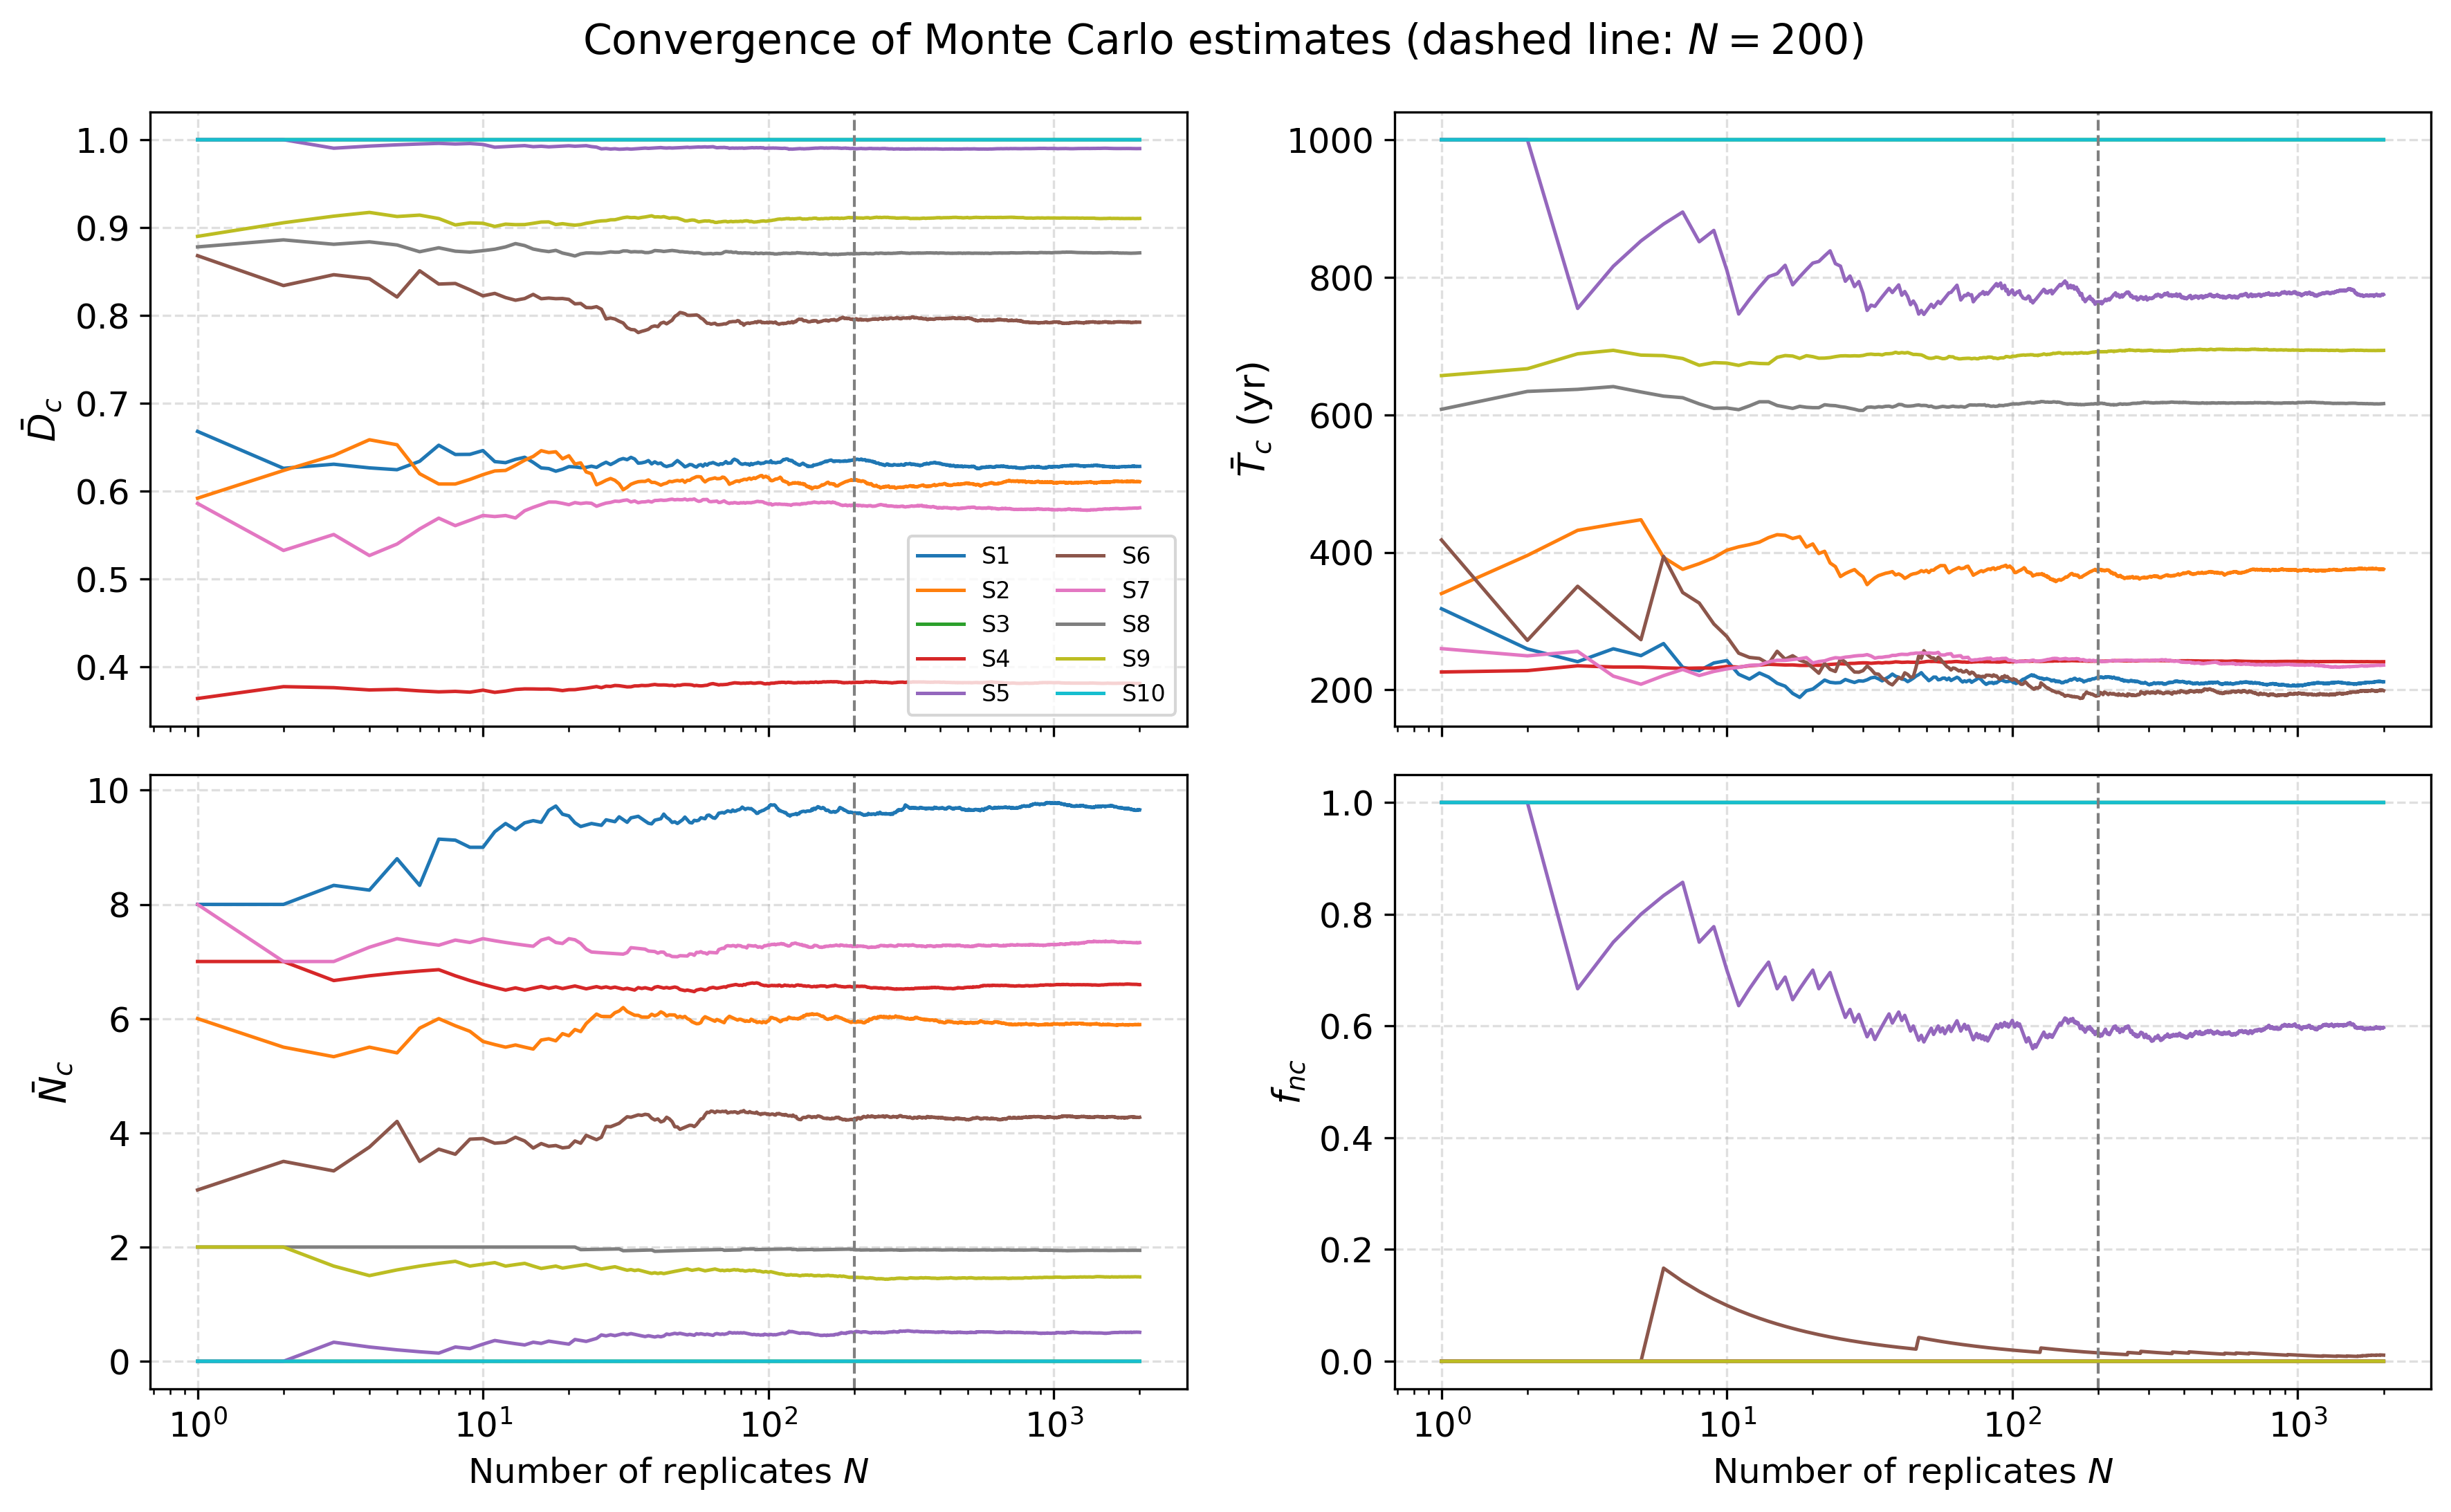
\includegraphics[width=\textwidth]{../figures/si/figureB_convergence.png}
\caption{Convergence of the cumulative Monte Carlo estimates of $\bar{D}_c$, $\bar{T}_c$, $\bar{N}_c$, and $f_{nc}$ with the number of replicates $N$, for all ten scenarios. The vertical dashed line marks $N = 200$, the ensemble size used in the main text.}
\label{fig:convergence}
\end{figure*}

\section{Individual simulated trajectories}\label{app:trajectories}

Because collapse events occur at different times in different runs, ensemble averages (and to a lesser extent medians) smooth the abrupt transitions that characterize individual histories. Supplementary Figure~\ref{fig:spaghetti} shows fifteen individual resource trajectories per scenario together with the median and the 5th--95th percentile envelope, making the timing variability and the sawtooth structure of the collapse-recovery cycles directly visible.

\begin{figure*}[htbp]
\centering
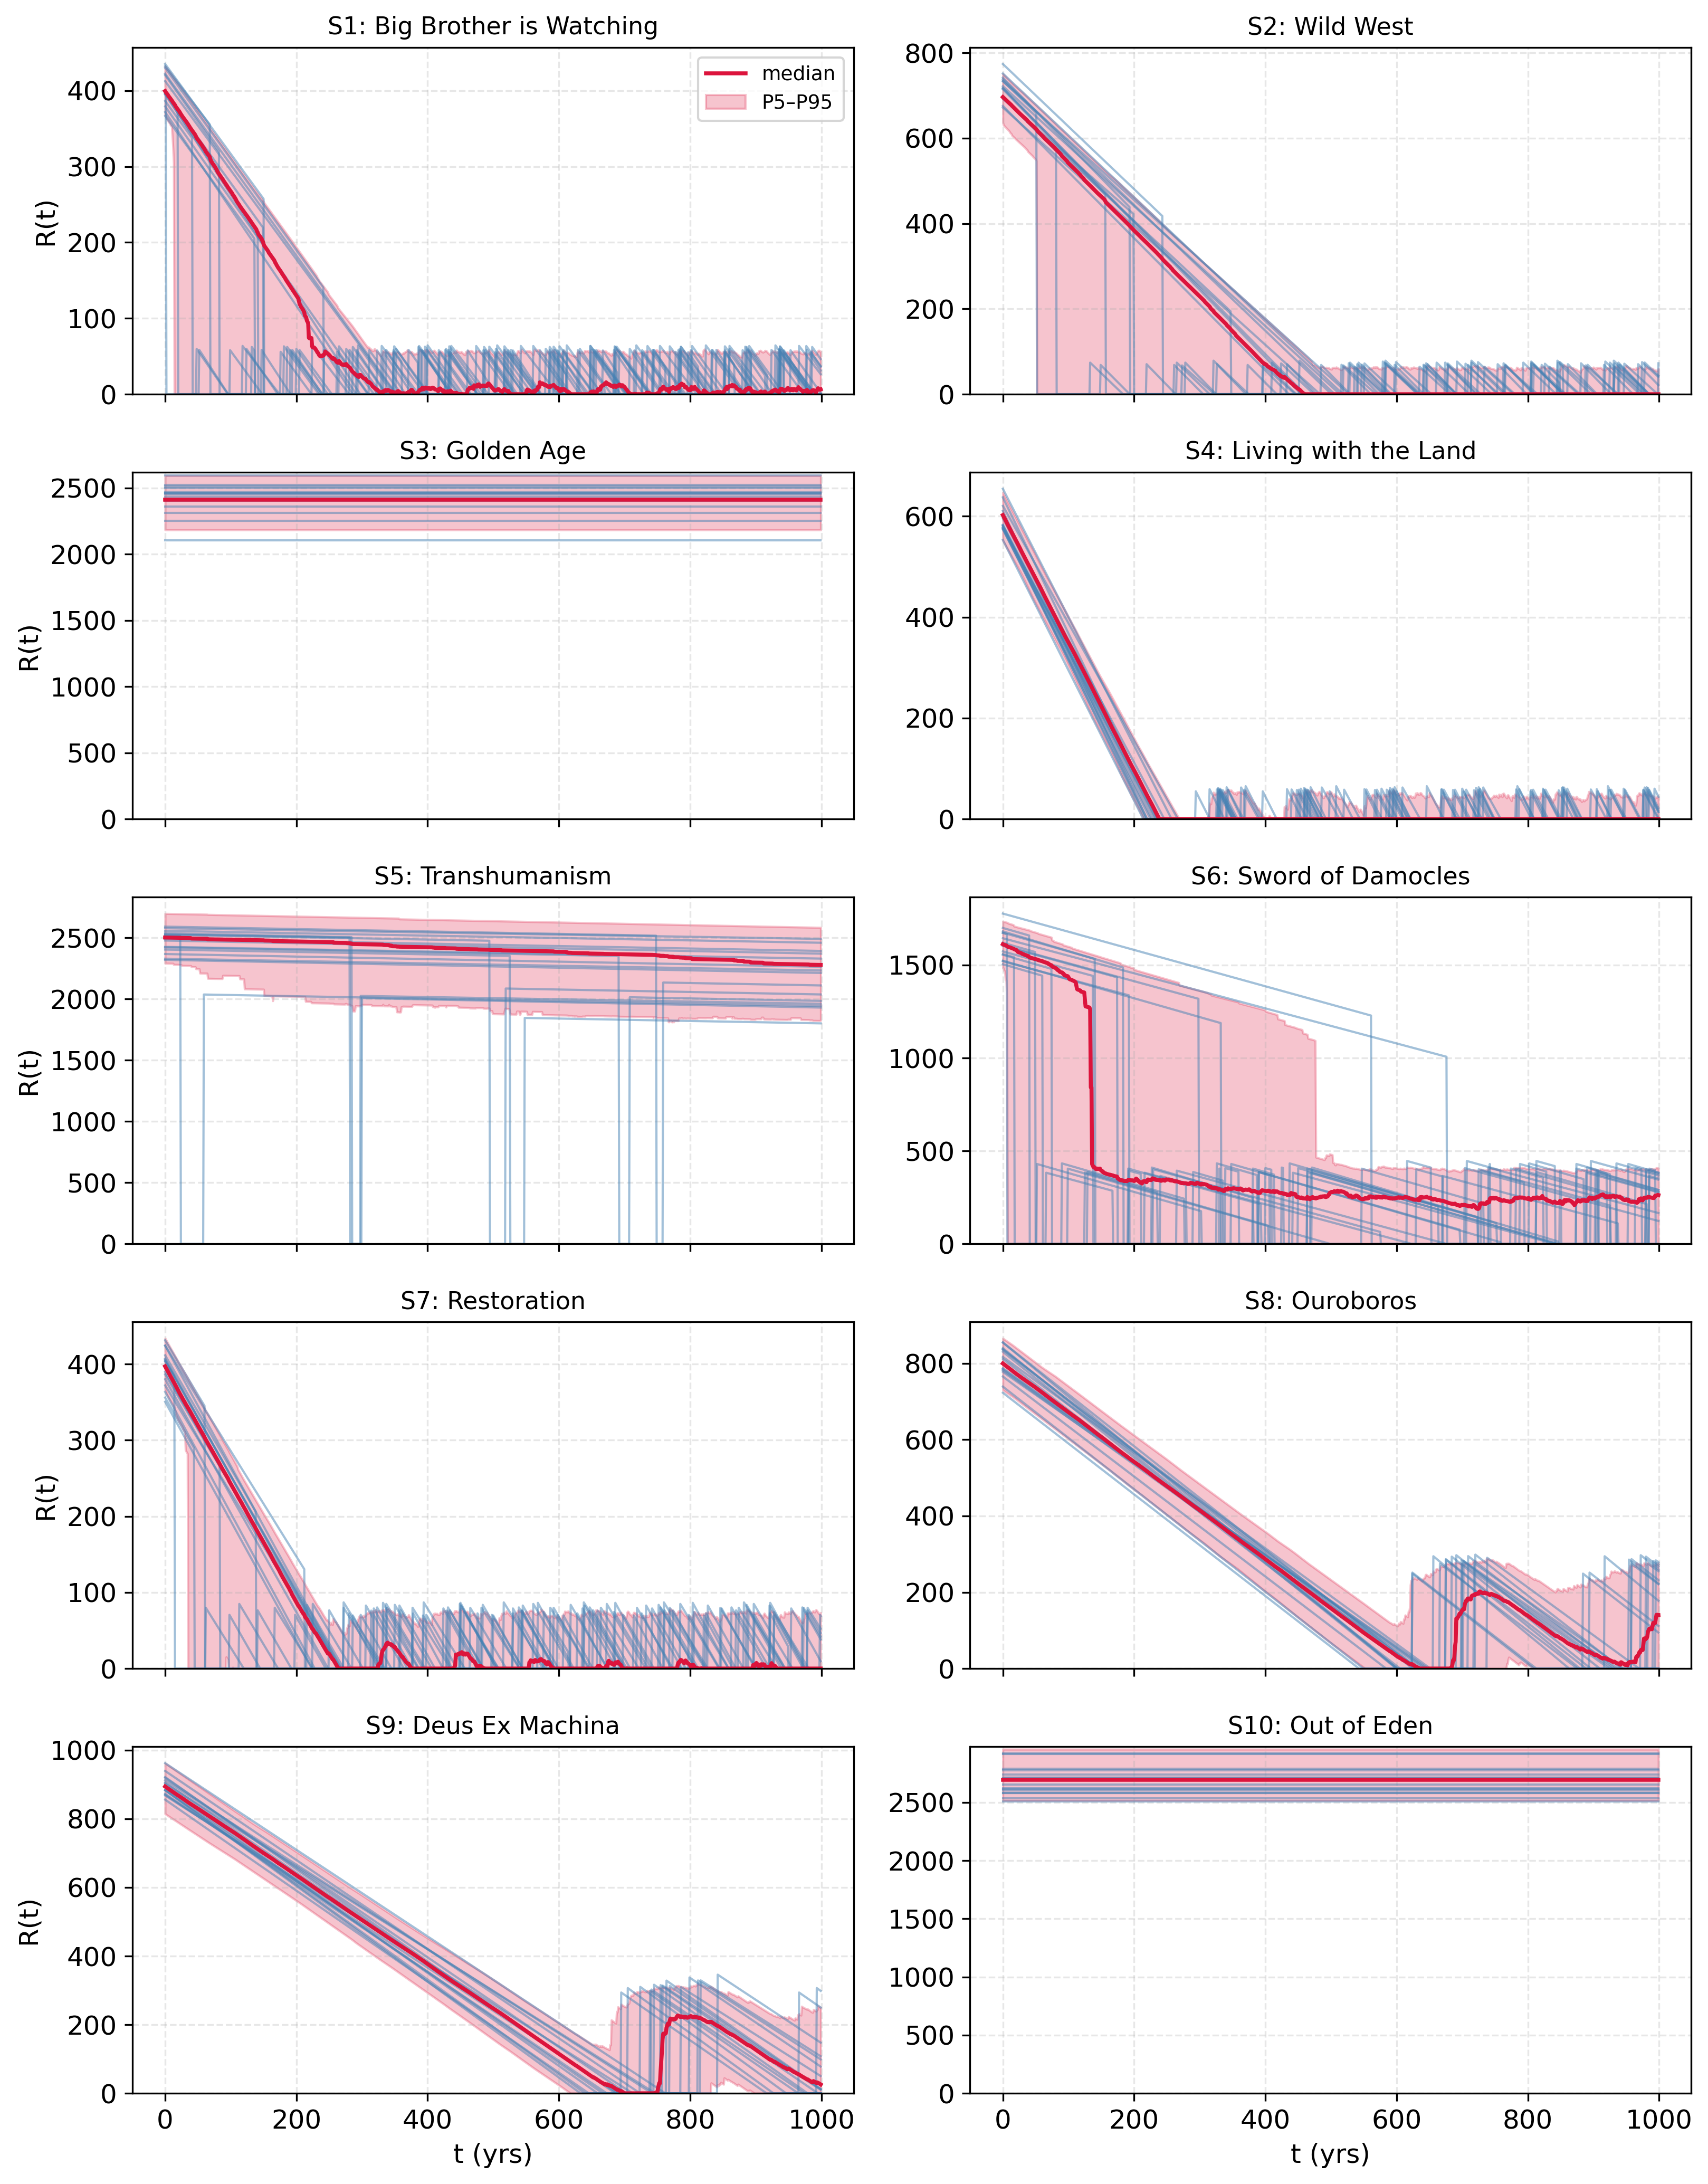
\includegraphics[width=0.95\textwidth]{../figures/si/figureA_trajectories.png}
\caption{Individual resource trajectories $R(t)$ (thin blue lines; 15 randomly selected replicates per scenario), median (red line), and 5th--95th percentile envelope (shaded; 200 replicates) for each of the ten scenarios.}
\label{fig:spaghetti}
\end{figure*}

\section{Simulation-horizon dependence and asymptotic duty cycle}\label{app:horizon}

To test whether the reported duty cycles are artifacts of the 1000-year simulation window, we re-ran all scenarios with horizons of 3,000 and 10,000 years (300 replicates each; Supplementary Figure~\ref{fig:horizon}). For the collapse-prone scenarios, the duty cycle decreases with horizon length and converges toward a stationary value, because the finite 1000-year window includes the favorable initial transient during which the full initial stock $R_0$ is being depleted, whereas the long-run dynamics are governed by the recurring cycle of partial recovery and re-depletion. The stationary value follows in closed form. In the cyclic regime, each cycle consists of an active phase, which lasts until the recovered stock $r_f R_0$ is depleted at rate $\delta$ or a hazard strikes, followed by a dormant phase of duration $r_d$. The depletion time is $\tau = r_f R_0 / \delta$, and with aggregate hazard exposure $h$ the expected active-phase duration is $t_{\mathrm{act}} = (1 - e^{-h\tau})/h$ (reducing to $\tau$ as $h \to 0$), giving
\begin{equation}
D_c^{\infty} = \frac{t_{\mathrm{act}}}{t_{\mathrm{act}} + r_d} .
\label{eq:dcinf}
\end{equation}
Table~\ref{tab:asymptotic} compares the simulated duty cycles at 1,000 and 10,000 years with Eq.~\eqref{eq:dcinf}; the analytic values agree with the 10,000-year simulations to within 0.025 for every collapse-prone scenario. The non-collapsing scenarios (S3, S10) remain at $D_c = 1$ at all horizons by construction ($\delta = 0$, $h = 0$), and S5 remains near-continuous ($D_c \approx 0.99$ at 10,000 yr) because its rare hazard-triggered collapses are followed by fast, nearly complete recovery. Two conclusions follow. First, the duty-cycle mechanism is not an artifact of the window length: it persists, in strengthened form, at horizons of $10^4$ years. Second, Eq.~\eqref{eq:dcinf} provides a window-independent characterization of intermittency that can be applied directly to the effective detectability duration $L_{\mathrm{eff}} = D_c L$ for civilizations of arbitrary lifespan $L$.

\begin{table}[htbp]
\centering
\caption{Simulated duty cycles at 1,000 and 10,000 yr horizons (300 replicates each) and the analytic asymptotic value of Eq.~\eqref{eq:dcinf}, for the collapse-prone scenarios.}
\label{tab:asymptotic}
\begin{tabular}{lccc}
\toprule
Scenario & $\bar{D}_c$ (1 kyr) & $\bar{D}_c$ (10 kyr) & $D_c^{\infty}$ (analytic) \\
\midrule
S1 & 0.631 & 0.555 & 0.537 \\
S2 & 0.620 & 0.420 & 0.394 \\
S4 & 0.382 & 0.215 & 0.194 \\
S6 & 0.795 & 0.776 & 0.776 \\
S7 & 0.578 & 0.479 & 0.464 \\
S8 & 0.872 & 0.767 & 0.755 \\
S9 & 0.913 & 0.786 & 0.776 \\
\bottomrule
\end{tabular}
\end{table}

\begin{figure*}[htbp]
\centering
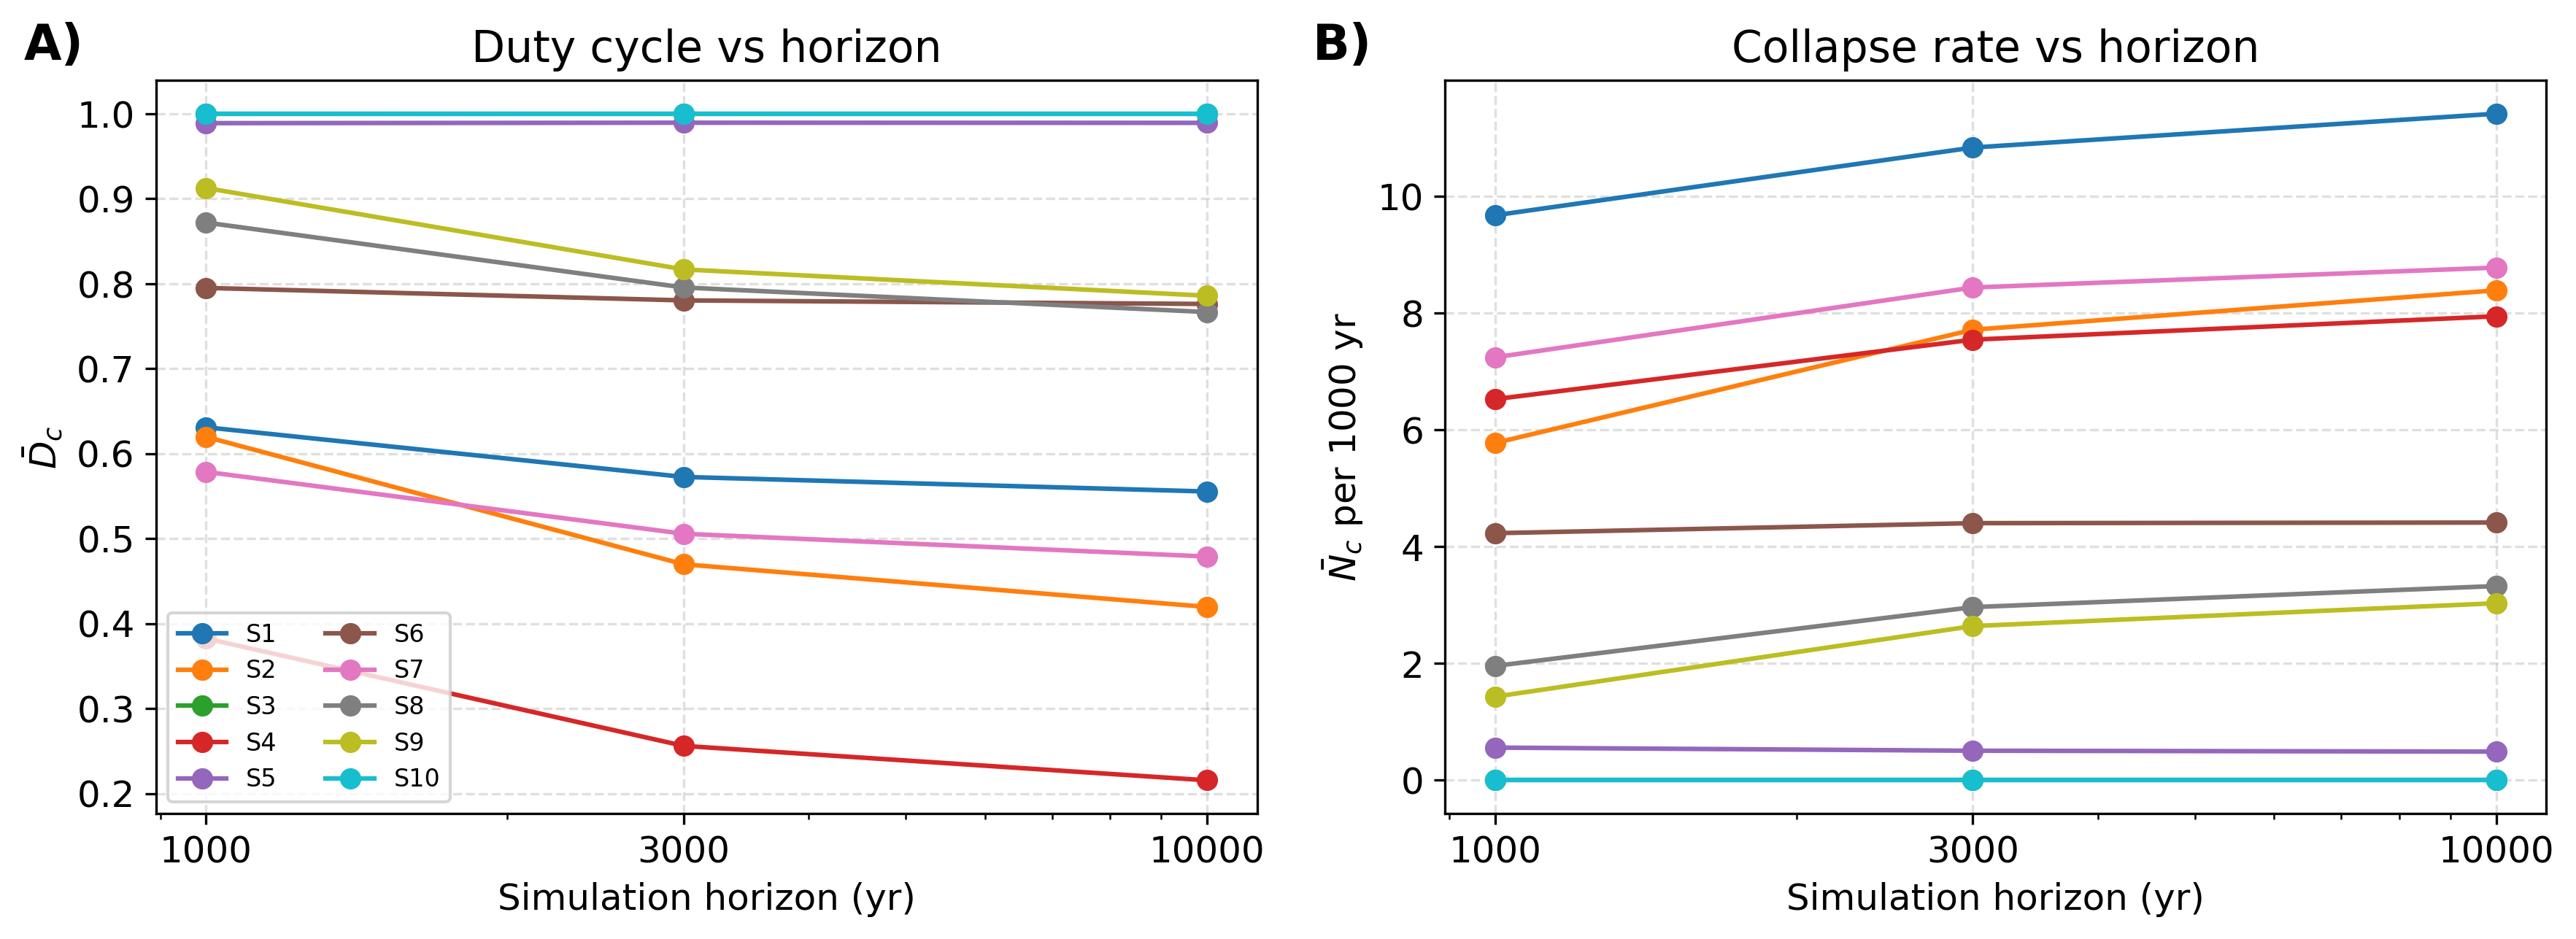
\includegraphics[width=\textwidth]{../figures/si/figureC_horizon.png}
\caption{(A) Mean duty cycle and (B) mean number of collapse events per 1000 years as a function of the simulation horizon (1,000, 3,000, and 10,000 yr; 300 replicates each).}
\label{fig:horizon}
\end{figure*}

\section{Robustness of the duty cycle to the ON threshold}\label{app:threshold}

The main-text analysis defines a civilization as ON when $R(t) > 0$. Supplementary Figure~\ref{fig:threshold} shows the duty cycle recomputed under the stricter criterion $R(t) > R_{\min}$, with $R_{\min}$ set to 2\%, 5\%, and 10\% of the scenario's initial stock (the dynamics are unchanged; only the activity criterion applied to the stored trajectories varies). As expected, stricter thresholds lower the duty cycle of the scarcity-driven scenarios, by up to 0.13 at the 5\% threshold and up to 0.28 at the 10\% threshold (largest for S1 and S2, whose trajectories spend long stretches at low resource levels), while leaving the abundant scenarios (S3, S5, S10) unaffected. The grouping of scenarios into continuous, intermediate, and strongly intermittent regimes, and every qualitative conclusion drawn from it, is preserved at all thresholds considered.

\begin{figure}[htbp]
\centering
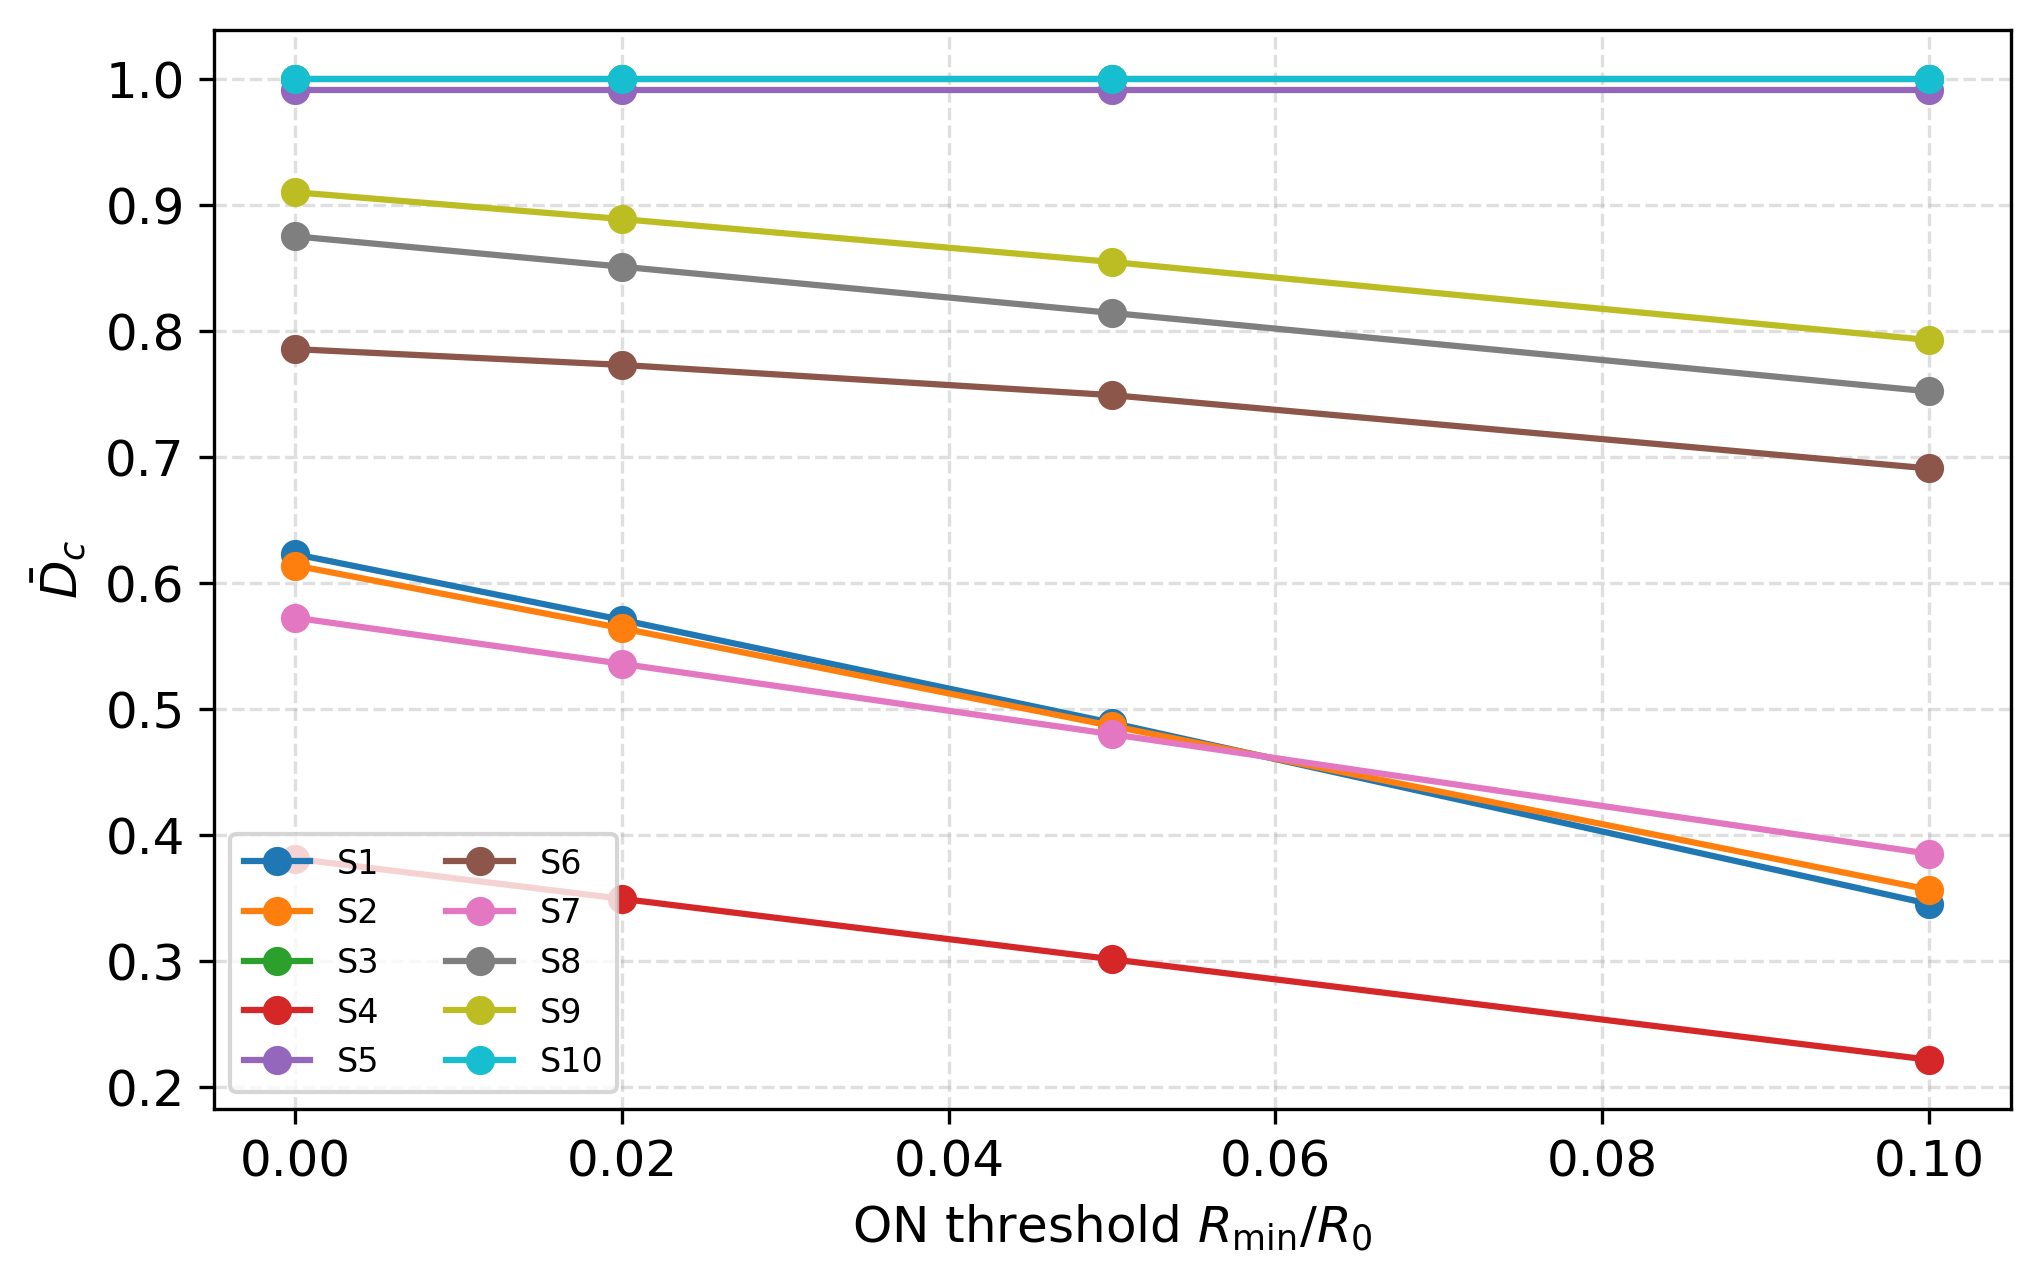
\includegraphics[width=0.75\columnwidth]{../figures/si/figureD_threshold.png}
\caption{Mean duty cycle as a function of the ON threshold $R_{\min}/R_0$, for all scenarios (200 replicates).}
\label{fig:threshold}
\end{figure}

\section{Two-parameter collapse maps for all collapse-prone scenarios}\label{app:2dmaps}

Supplementary Figure~\ref{fig:2dmaps} generalizes the two-parameter analysis of Figure~2B of the main text to every collapse-prone scenario, mapping the mean number of collapse-recovery cycles over the $(r_f, \delta)$ plane with all other parameters held at scenario baselines (20 hazard replicates per grid point). All scenarios display the same qualitative structure: a high-cycling regime at low recovery fraction and high depletion, a regime boundary along which modest parameter shifts change the cycle count, and suppression of collapse at high $r_f$ and low $\delta$. Differences among panels reflect the scenarios' baseline stocks and exposures (e.g., the map for S6 is flattened by its dominant exogenous hazard).

\begin{figure*}[htbp]
\centering
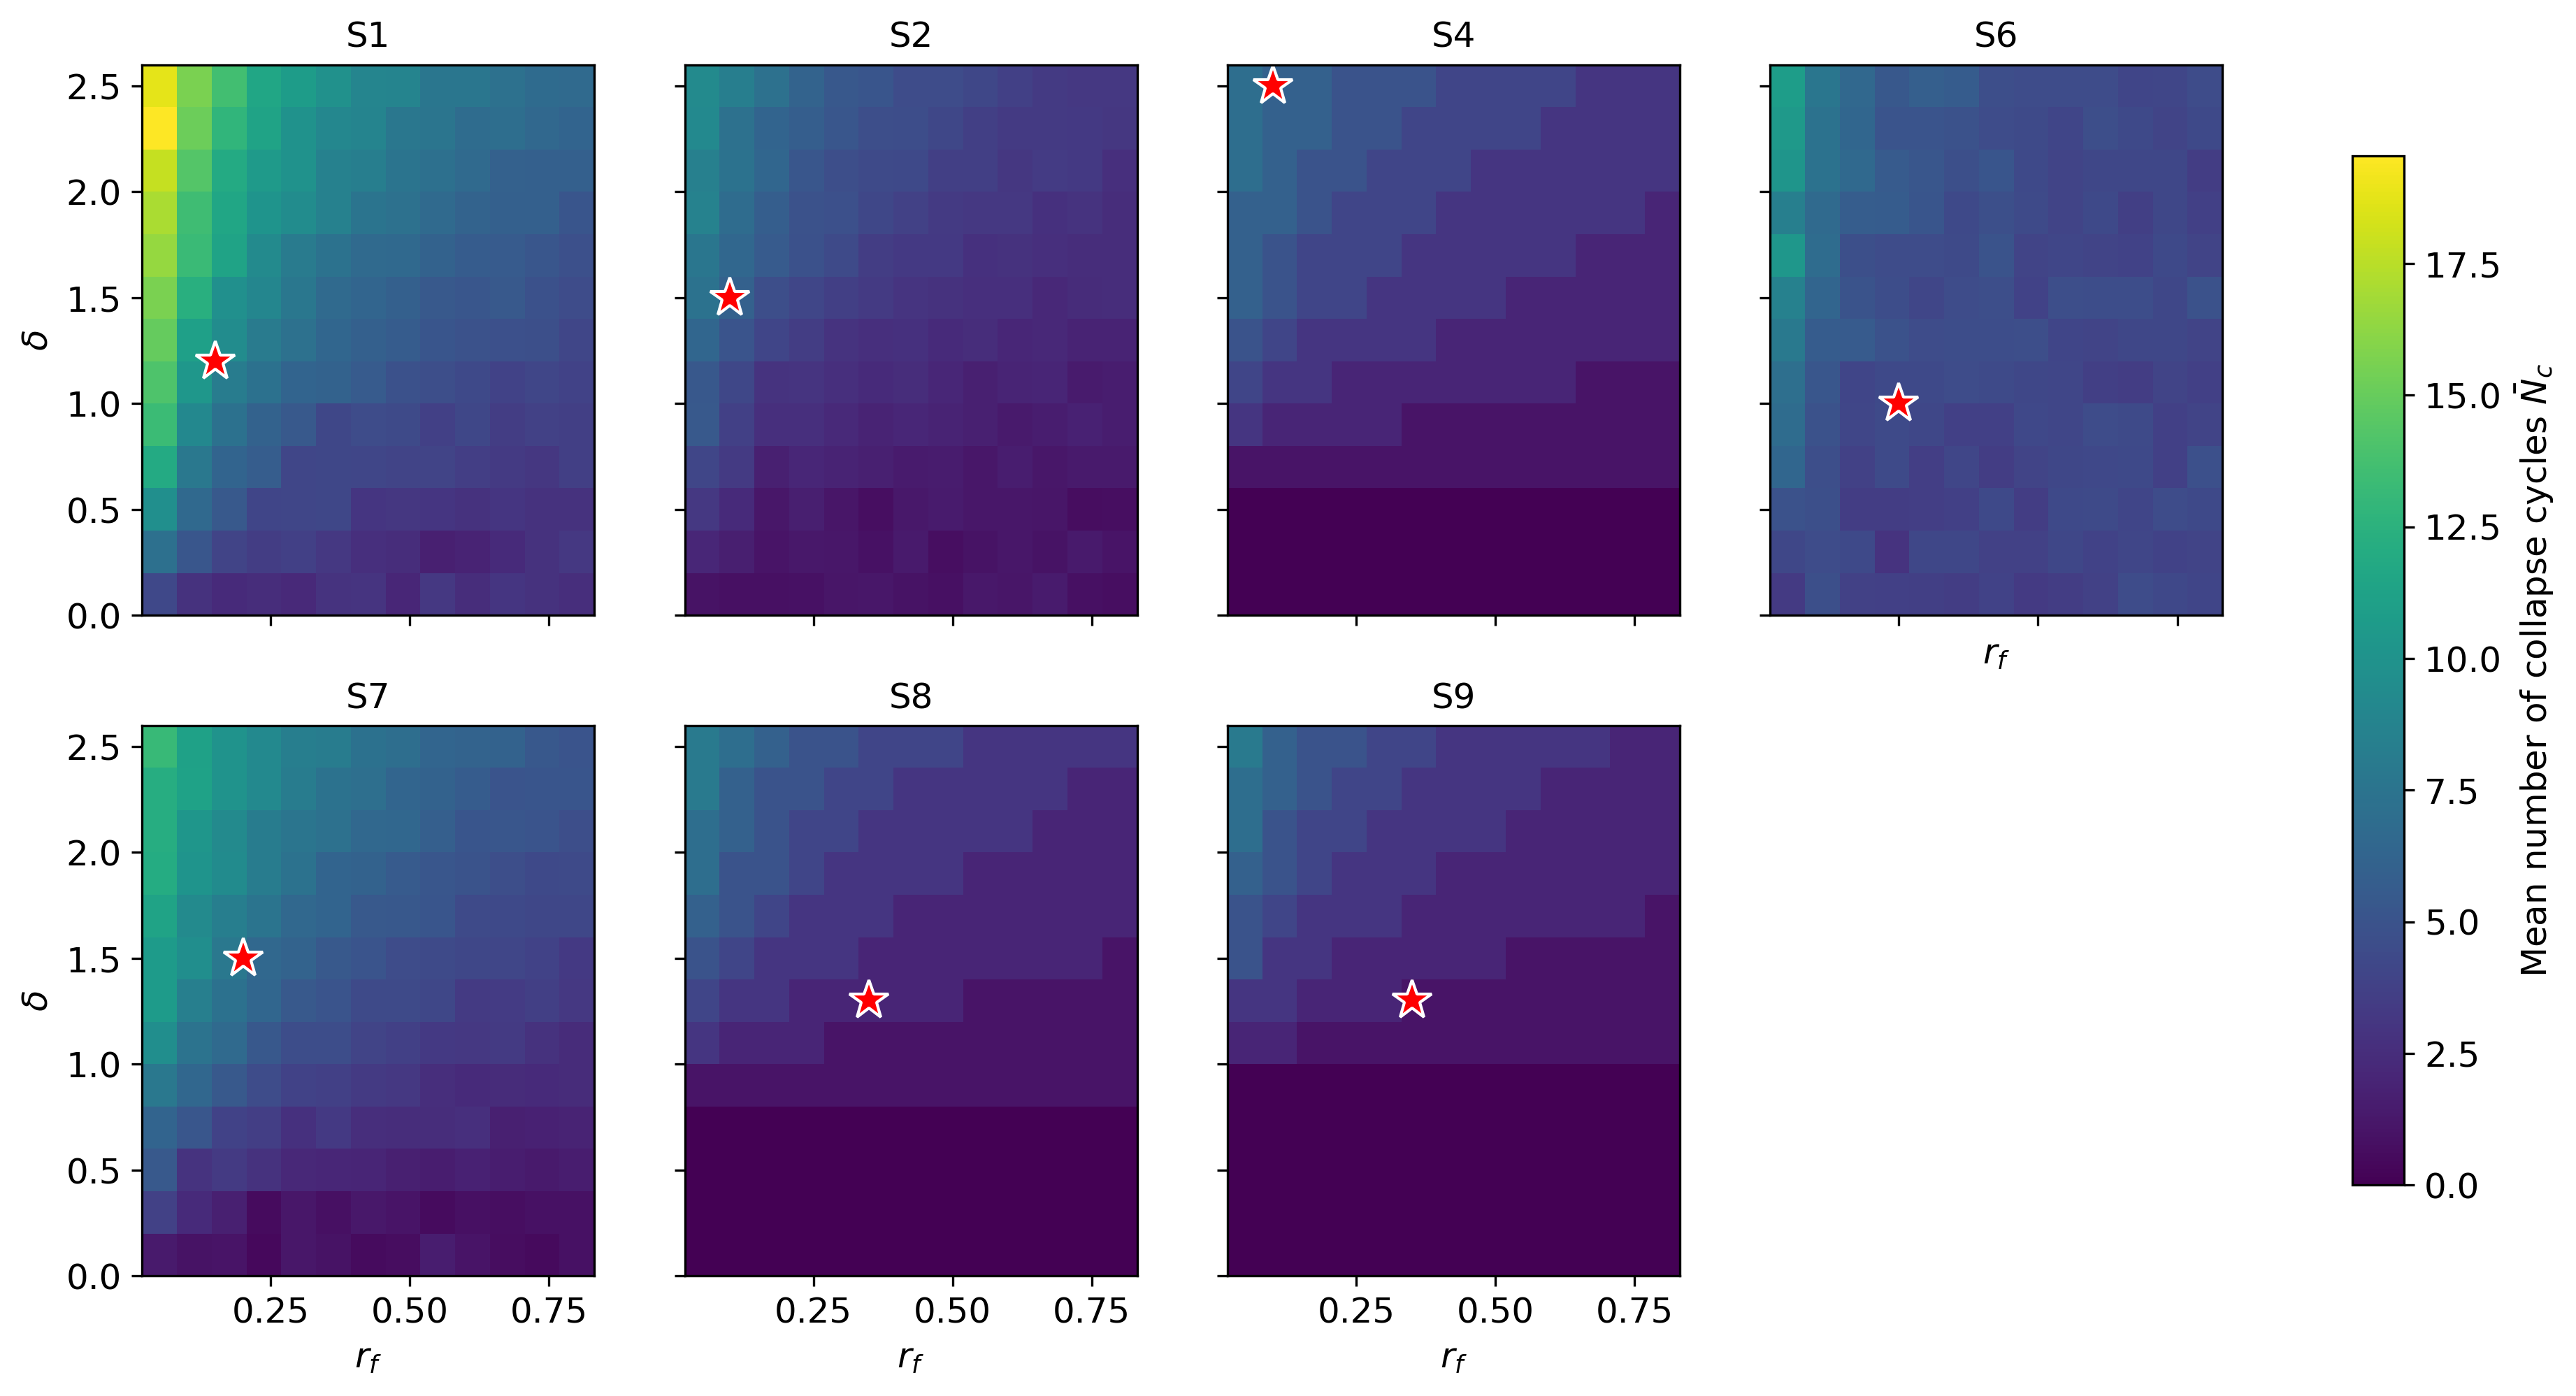
\includegraphics[width=\textwidth]{../figures/si/figureE_2dmaps.png}
\caption{Mean number of collapse-recovery cycles over the $(r_f, \delta)$ plane for each collapse-prone scenario (20 hazard replicates per grid point). Red stars mark baseline parameter combinations.}
\label{fig:2dmaps}
\end{figure*}

\section{Growth-law invariance and technology coupling}\label{app:growth}

\paragraph{Invariance.} In the baseline model, technological capacity $T(t)$ does not feed back on resource dynamics: collapse timing, dormancy, and recovery are functions of $R(t)$ alone. All four outcome metrics are therefore strictly invariant to the functional form chosen for technological growth. We verified this numerically by re-running the full Monte Carlo ensemble with identical random seeds under linear (baseline), bounded-exponential, and logistic growth laws: the resulting values of $\bar{D}_c$, $\bar{T}_c$, $\bar{N}_c$, and $f_{nc}$ are identical to machine precision. The choice of a linear growth law thus affects the reported technology trajectories $T(t)$, but none of the collapse-recovery statistics on which the paper's conclusions rest.

\paragraph{Coupling.} The substantive question is therefore not the shape of the growth law but the absence of technology-resource feedback. To probe it, we implemented two coupled variants. In the \emph{efficiency coupling}, technology reduces the effective depletion rate, $\delta_{\mathrm{eff}} = \delta / (1 + \gamma_\delta (T - 1))$, representing efficiency gains from accumulated capability. In the \emph{recovery coupling}, technology raises the post-collapse recovery fraction, $r_{f,\mathrm{eff}} = \min[1, r_f (1 + \gamma_r (T - 1))]$, representing the use of retained capability to rebuild. Supplementary Figure~\ref{fig:coupling} shows the mean duty cycle of each collapse-prone scenario as the coupling strengths are swept over $\gamma \in \{0, 0.1, 0.25, 0.5, 1.0\}$. The efficiency coupling raises duty cycles modestly and monotonically (by at most 0.06 at $\gamma_\delta = 0.5$), while the recovery coupling has almost no effect (at most 0.01): because each collapse multiplies $T$ by $c_f$, technological capacity in the collapse-prone regimes is eroded back toward or below its initial value before it can meaningfully boost recovery, a ratchet-limiting effect that is itself an instructive property of collapse-recovery dynamics. The ranking of scenarios by duty cycle is exactly preserved for $\gamma \leq 0.25$ in both variants and largely preserved at stronger couplings (rank correlation $\geq 0.79$ in all cases). We conclude that the paper's comparative conclusions are robust to moderate technology-resource feedback, while noting that strongly coupled models, in which technology expands the accessible stock $R_0$ itself, remain an important direction for future work (Section~7 of the main text).

\begin{figure*}[htbp]
\centering
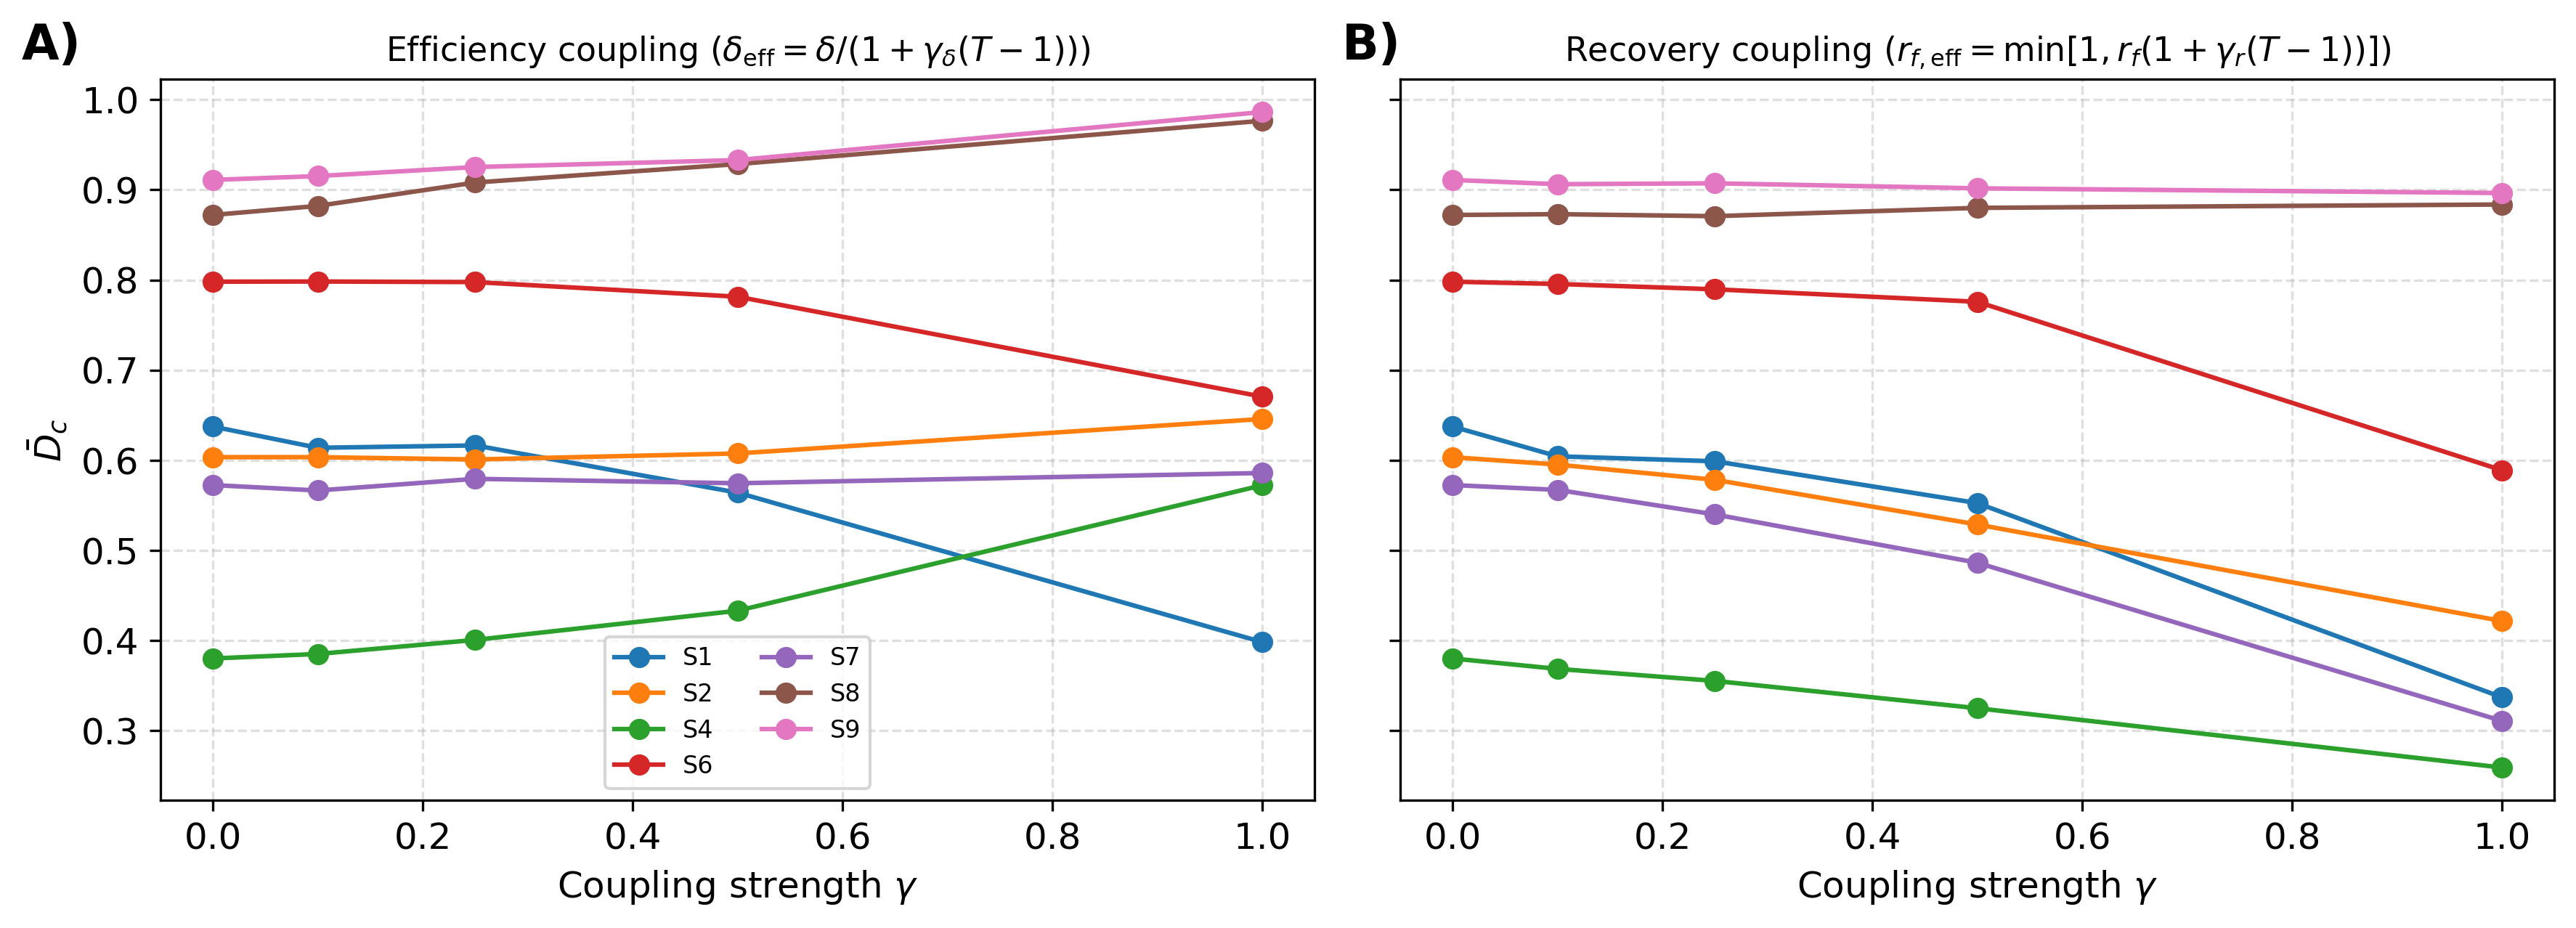
\includegraphics[width=\textwidth]{../figures/si/figureF_coupling.png}
\caption{Mean duty cycle of each collapse-prone scenario as a function of coupling strength $\gamma$ for (A) the efficiency coupling and (B) the recovery coupling (200 replicates per point).}
\label{fig:coupling}
\end{figure*}


\section{Global sensitivity analysis}\label{app:gsa}

Because one-at-a-time sweeps cannot capture interactions among simultaneously varying parameters, we complement them with a global sensitivity analysis. For each collapse-prone scenario we draw 400 Latin Hypercube samples over the full five-dimensional parameter space ($r_f$, $\delta$, $r_d$, $h$, $c_f$), spanning the same global bounds as Table~6 of the main text, and compute partial rank correlation coefficients (PRCC) of the outcome metrics with respect to each parameter (Supplementary Figure~\ref{fig:gsa}). The global analysis confirms the one-at-a-time picture while adding two refinements. First, when all parameters vary jointly across their full plausible ranges, the recovery delay $r_d$ emerges as an influence on the duty cycle comparable to $r_f$ and $\delta$ (PRCC between $-0.83$ and $-0.87$ across scenarios): its local effect around the scenario baselines is modest (Figure~5 of the main text), but over its full range it is a first-order control on continuity. Second, the analysis cleanly separates which parameters control which outcome: the time to first collapse $\bar{T}_c$ is governed almost exclusively by $\delta$ and $h$ (the recovery parameters $r_f$ and $r_d$ have PRCC magnitudes below 0.1, as they only act after the first collapse), whereas the duty cycle integrates both failure and recovery and therefore responds strongly to all four. The aggregate hazard exposure $h$ is the dominant driver in S6 for both outcomes, consistent with the one-at-a-time result, and the collapse survival fraction $c_f$ has negligible influence on all metrics in all scenarios (|PRCC| $\leq 0.12$), supporting its exclusion from the sweep figures. Two-parameter interaction maps over $(r_f, \delta)$ are also available for every collapse-prone scenario (Supplementary Figure~S5).

\begin{figure*}[htbp]
\centering
\centering
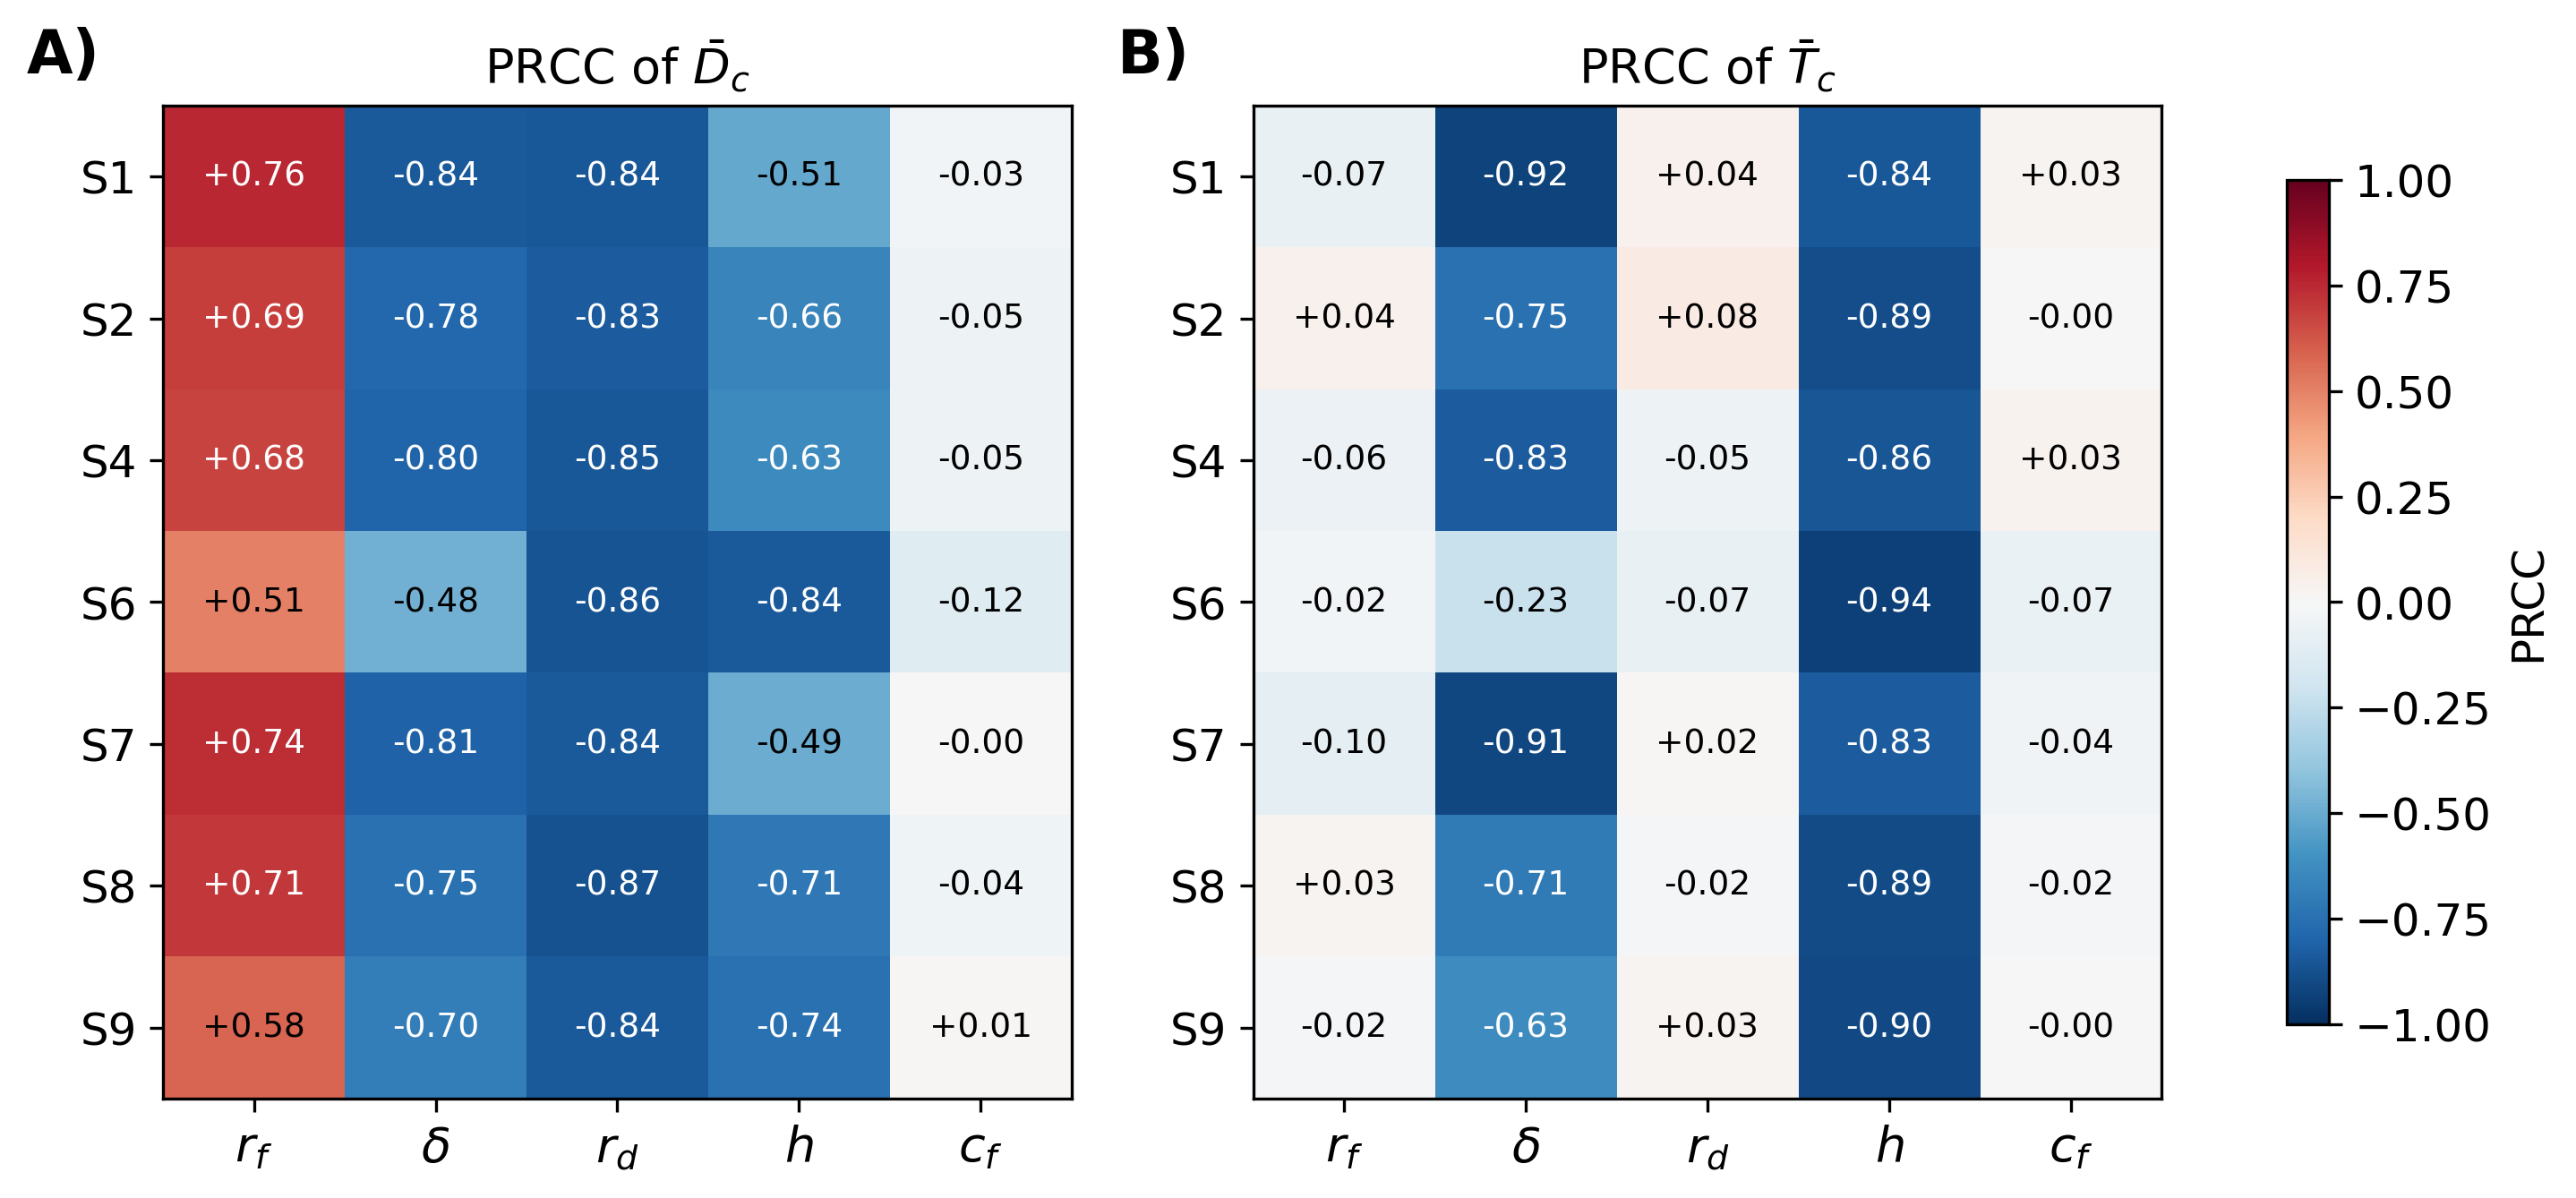
\includegraphics[width=\textwidth]{../figures/si/figure_gsa_prcc.png}
\caption{Global sensitivity analysis for all collapse-prone scenarios. Partial rank correlation coefficients (PRCC) of (A) the mean duty cycle $\bar{D}_c$ and (B) the mean time to first collapse $\bar{T}_c$ with respect to each model parameter, computed from 400 Latin Hypercube samples per scenario spanning the global bounds of Table~6 of the main text (plus $c_f \in [0.1, 1.0]$), with 25 hazard replicates per sample.}
\label{fig:gsa}
\end{figure*}

\end{document}
